
\chapter{弱监督分割方法及实现}
\section{引言}
机器学习在各种任务中取得了巨大成功,特别是在分类和回归等监督学习任务中。其中分割问题也可以归为分类问题,即对每一个像素进行分类。
%预测模型是从包含大量训练样本的训练数据集中学习,每个训练样本对应一个事件或对象。训练样本由两部分组成:一个描述对象的特征向量,以及一个表示真值输出的标签。
在分类任务中,标签表示训练样本所属的类别;在回归任务中,标签是一个与样本对应的实数值。大多数成功的技术,如深度学习,都需要含有真值标签的大规模训练数据集。然而,在许多任务中,由于数据标注过程的成本极高,很难获得强监督信息。尤其是在医学图像分割领域,获取图像真实值十分的耗时耗力而且容易出错。因此,此领域的研究者十分希望获得能够在弱监督前提下工作的机器学习技术。

目前的弱监督研究领域主要关注三种弱监督类型:不完全监督、不确切监督、以及不准确监督。第一类是不完全监督,即只有训练集的一个(通常很小的)子集是有标签的,其他数据则没有标签。这种情况发生在各类任务中。例如,在图像分类任务中,真值标签由人类标注者给出的。从互联网上获取巨量图片很容易,然而考虑到标记的人工成本,只有一个小子集的图像能够被标注。第二类是不确切监督,即图像只有粗粒度的标签,比如说对图像只有图像类别级的标签。第三种是不准确的监督,模型给出的标签不总是真值。出现这种情况的常见原因有,图片标注者不小心或比较疲倦,或者某些图片就是难以分类。

本文所研究的弱监督属于第二类不确切监督,在接下来的文章当中,本文将不再区别弱监督的类别,而将其默认指代为不确切监督。

\section{方法框架}
本节详细介绍了算法的框架,如图\ref{fig:framework}。在这个框架中,本文采取了一种名为“既见森林,又见树木”的策略。 “森林”是指白癜风本身的特征,“树”是指每个患者的特定皮肤状况(例如,健康的肤色和白癜风的脱色程度)。为了了解白癜风本身的本质,本文训练了一个深度卷积神经网络用于Vit2019的分类。通过查看树,本文利用在推理阶段从输入图像中提取的信息,首先将其分割为超像素,然后在超像素级别上进行提取特征。为了实现“既见森林,又见树木”,本文结合从两方面获得的知识,然后将其作为有用的先验知识引入显着性传播过程。
\begin{figure}[htbp]
\begin{center}
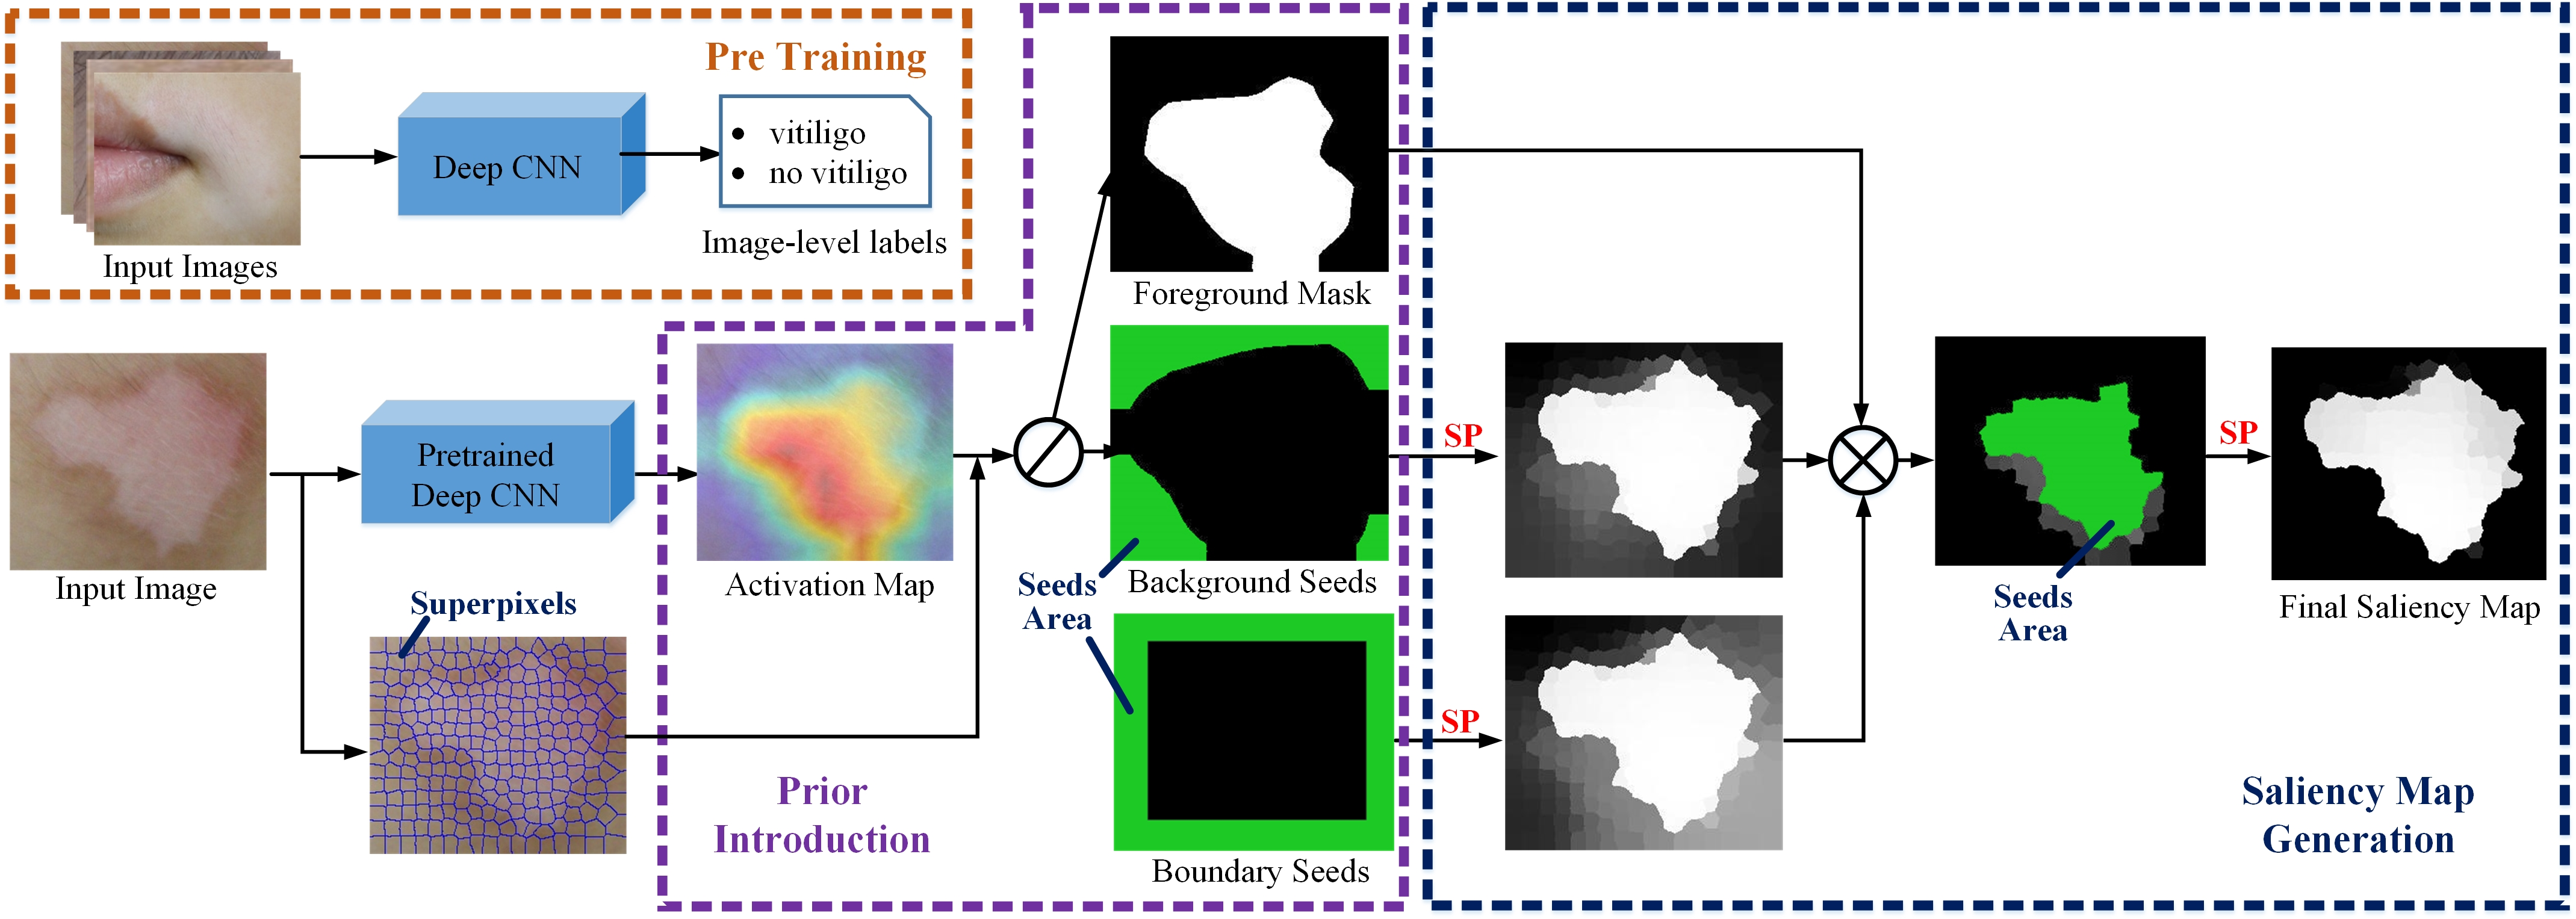
\includegraphics[width=\linewidth]{CNNandSuperPixelModelGraph3.jpg}
\end{center}
   \caption{本文弱监督算法的框架。在第一阶段,训练深度卷积神经网络以识别图像类别。当给定输入图像时,将其分割成超像素;另一方面,使其通过训练好的分类网络以获得激活图。在先验的引入阶段,激活图通过给出种子区域来提供用于显着性传播的先验知识。在显着图生成阶段,本文首先生成一个粗显着图,然后对其进行细化以获得最终显着图. $ \oslash $表示阈值操作。SP 表示在\ref{sec:propagation}节中详述的显着性传播过程。}
\label{fig:framework}
\end{figure}

在接下来的小节中,将详细说明如何通过预先训练的模型获取激活图,如何在超像素上构建图模型,如何通过传播过程生成最后的显著图。

\subsection{预训练分类模型}

本文训练CNN模型来对Vit2019数据集中的图像进行分类,通过简单地在全连接层之前对卷积特征图执行全局平均池化(GAP),利用CNN的副产品---激活图---粗略定位白癜风区域。分类器的准确性可以在一定程度上反映显着图的质量\cite{simonyan2013deep, zhou2016learning}。在这项工作中,本文训练了一个分类错误率为4.27\%ResNet \cite{He_2016_CVPR}的模型。在实践中,当收集新一批图像时,可以使用迁移学习或者微调先前的模型而不是从头开始重新训练。

\subsection{生成类激活图}
只在输出层前(用于分类的softmax)使用全局平均池化层,并将它们作为得出分类的全连接层的特征。通过这种简单的连接结构,可以把图片中的重要区域用输出层权重映射回卷积层特征的方式标记出来,称这种技术为类激活映射(CAM)。如图\ref{fig:CAM}所示,全局平均池化层输出最后一个卷积层的每个单元的特征图的平均值。这些值的加权总和用于生成最后的输出。也可以说,计算最后一个卷积层特征图的加权总和来获得CAM。下面使用更形式化的方式来描述。
\begin{figure}[htbp]
\begin{center}
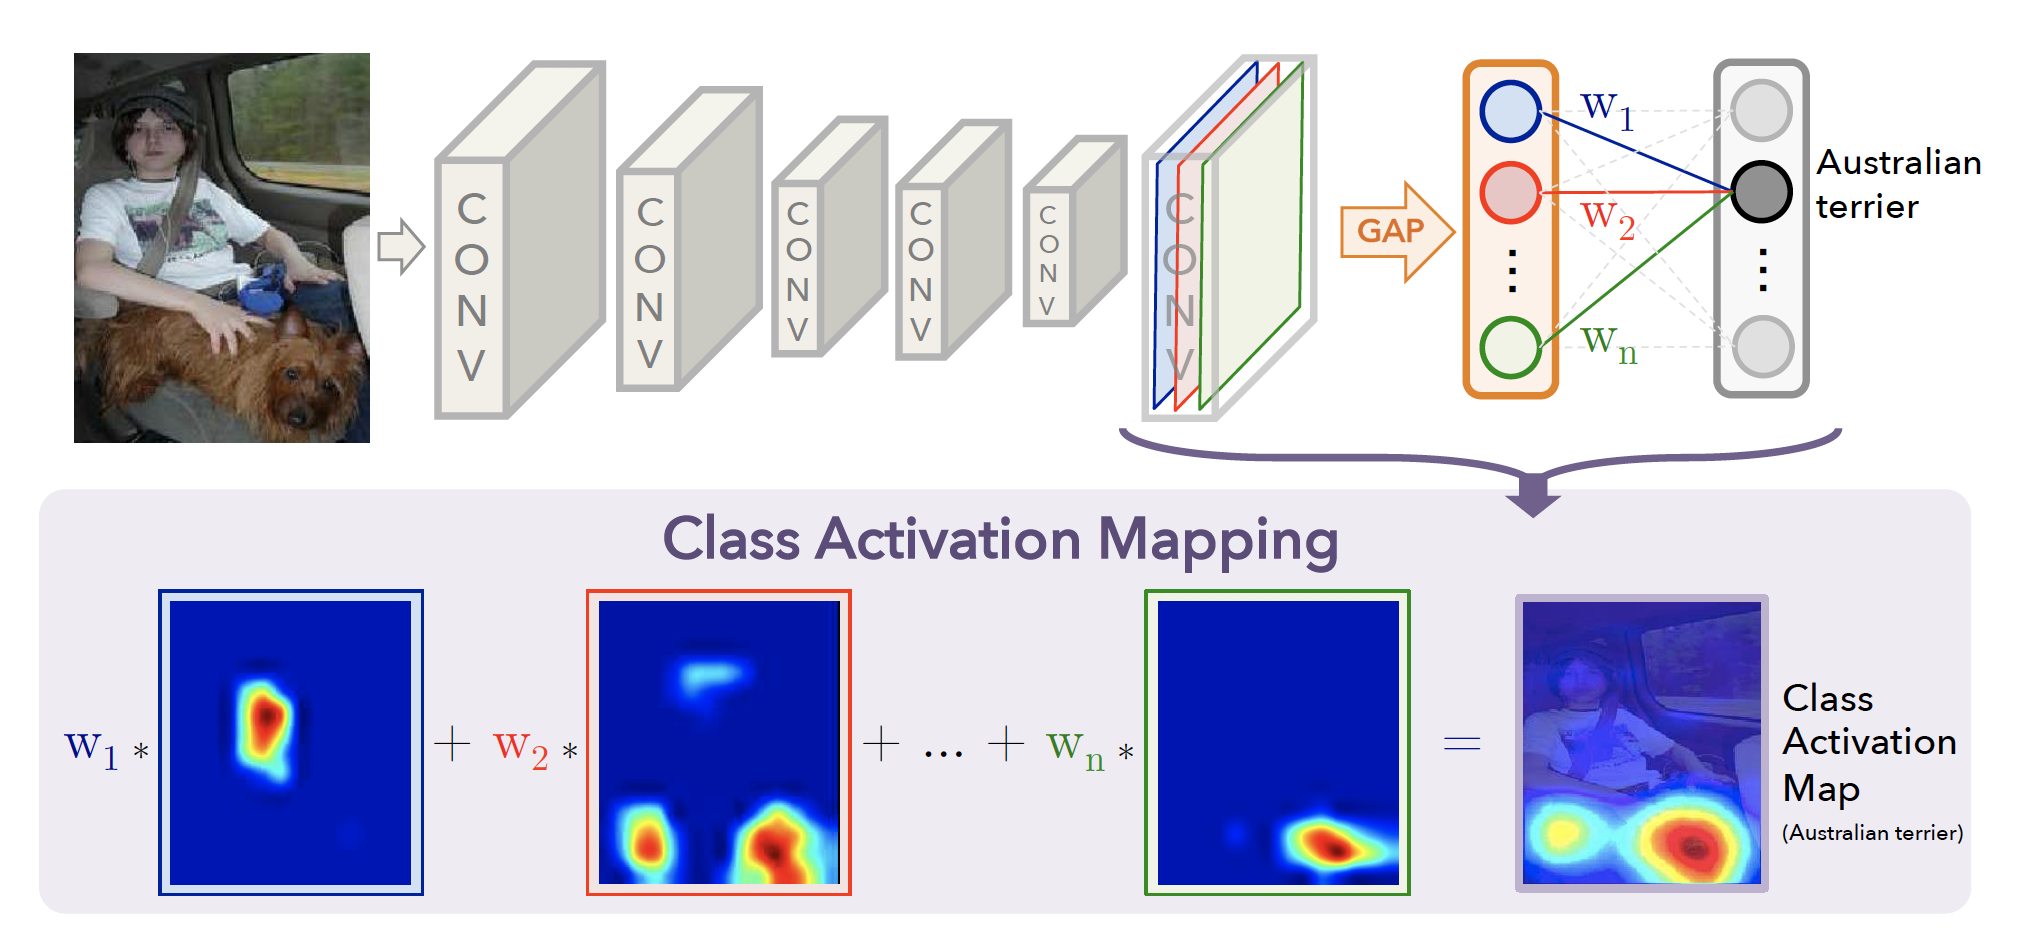
\includegraphics[width=0.9\linewidth]{CAM.png}
\end{center}
\caption{类激活图生成\cite{zhou2016learning}。将预测的类别得分映射回先前的卷积层以生成类显著图(CAMs)。CAM突出了类特定的判别区域。}
\label{fig:CAM}
\end{figure}

对于一个给定的图,用$f_k(x, y)$代表最后一个卷积层在空间坐标$(x,y)$中单元$k$的激活值。然后,对于每个单元$k$,通过GAP后的结果为:
\begin{equation}
\label{eq:chap4_1}
F_k=\sum_{x, y} f_{k}(x, y)
\end{equation}
对于每个类$c$,输入softmax的$S_c$为:
\begin{equation}
\label{eq:}
\sum_{k} w_{k}^{c} F_{k}
\end{equation}
$w_k^c$代表单元$k$对应的类$c$的权重。实际上,$w_k^c$就是$F_k$对类$c$的重要性。最后类$c$的sotfmax输出:
\begin{equation}
\label{eq:}
P_c=\frac{\exp \left(S_{c}\right)}{\sum_{c} \exp \left(S_{c}\right)}
\end{equation}
这里忽略偏差项:明确地把softmax的偏差项设置为0。因为它几乎对分类表现没有影响。
把公式\ref{eq:chap4_1}带入$S_c$,得
\begin{equation}
\label{eq:}
S_{c}=\sum_{k} w_{k}^{c} \sum_{x, y} f_{k}(x, y)=\sum_{x, y} \sum_{k} w_{k}^{c} f_{k}(x, y)
\end{equation}
这里用$M_c$定义类别$c$的CAM,则空间中每个元素为
\begin{equation}
\label{eq:}
M_{c}(x, y)=\sum_{k} w_{k}^{c} f_{k}(x, y)
\end{equation}
因此就有
\begin{equation}
\label{eq:}
S_{c}=\sum_{x, y} M_{c}(x, y)
\end{equation}
所以$M_c(x,y)$直接表明了像素$(x,y)$对网络将图片归类为$c$的贡献。

根据先前的研究\cite{zeiler2014visualizing},研究者都希望用一些可视化方法看到每个被激活的单元的激活区域,$f_k$就是这种可视化方法。简单说CAM就是不同空间区域的线性加权可视化。将类激活图的大小改变成输入图片的大小,就能清楚地看出与特定类最相关的区域。

图\ref{fig:cam}展示了一些作用于白癜风图像上的输出,可以看到属于白癜风区域已经高亮,这说明是这些区域帮助网络将此图片分类为白癜风图片。换一种说法,网络在接收到这张图片后,注意力集中在热度图的红色区域。
\begin{figure}[htbp]
\begin{center}
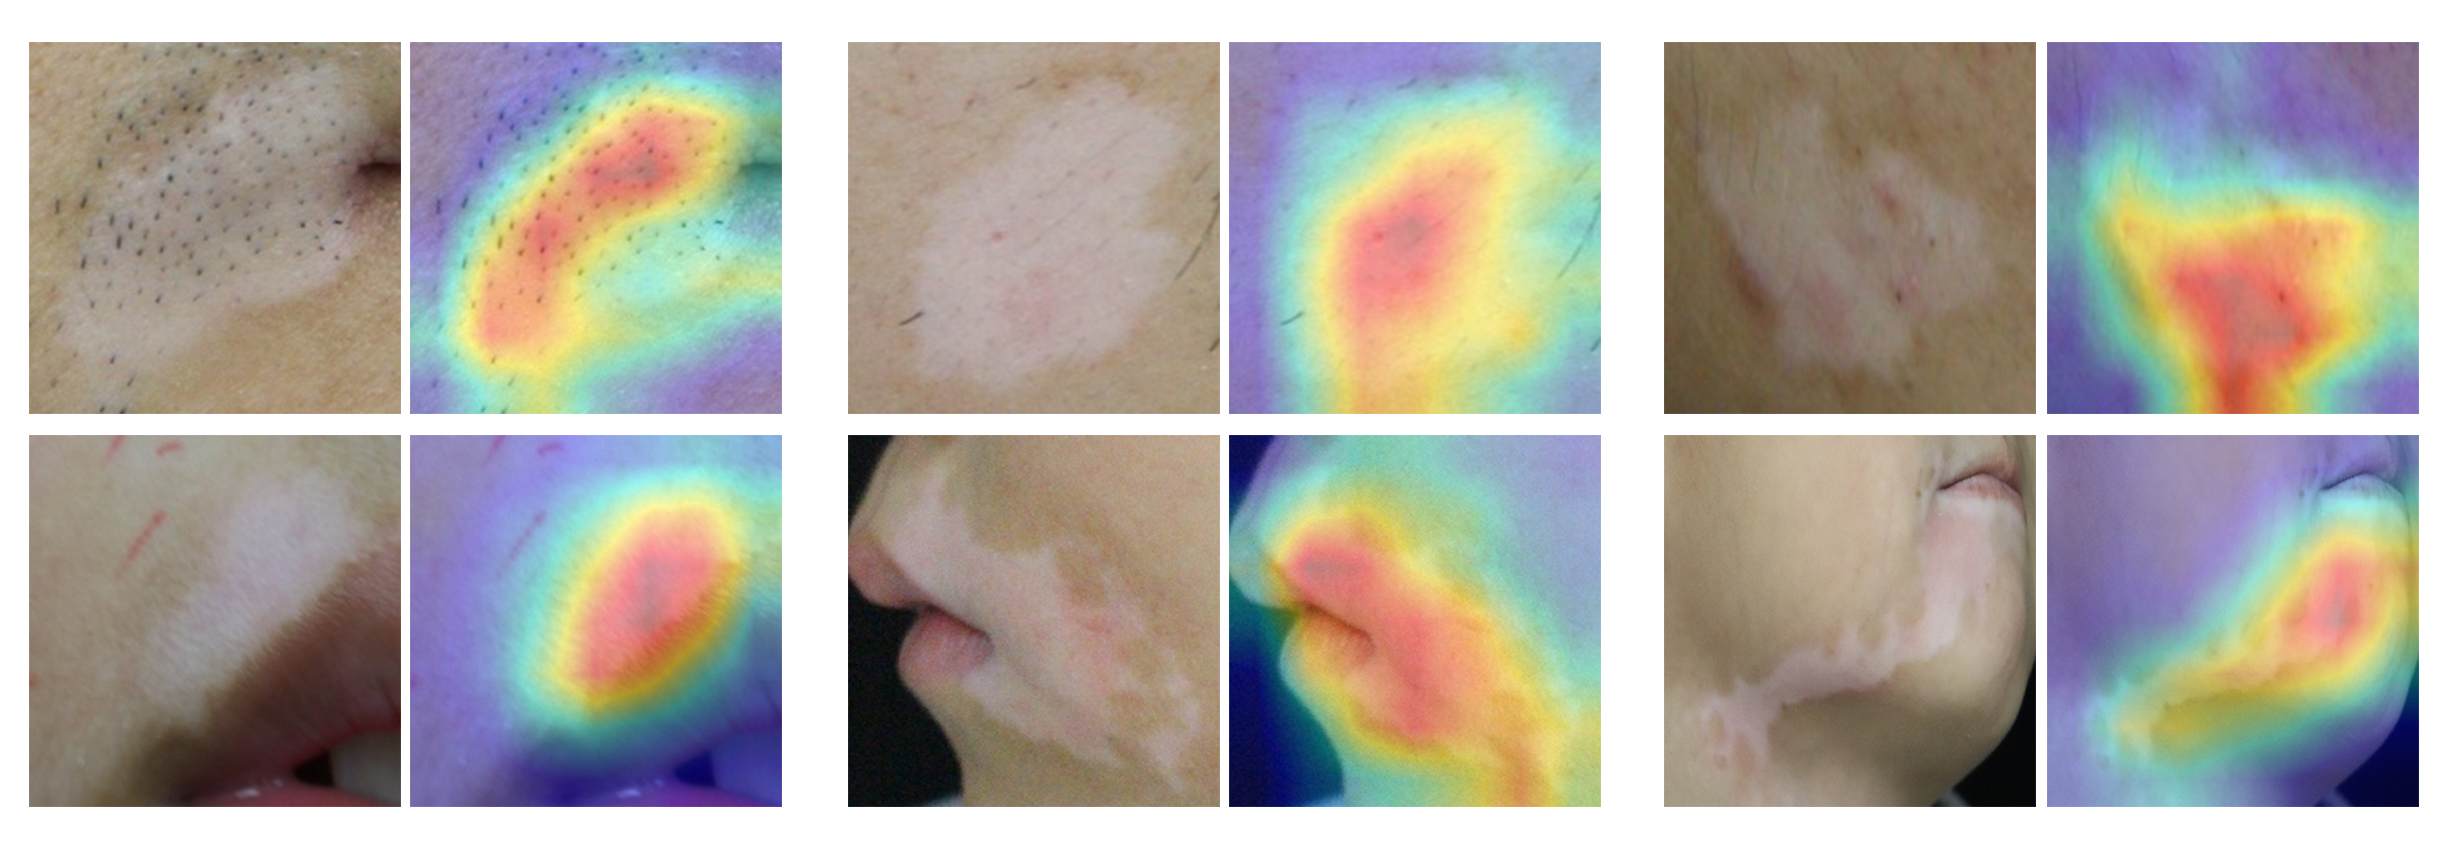
\includegraphics[width=\linewidth]{cam.jpg}
\end{center}
\caption{显著图的示例。蓝色区域表示低的激活值;而红色区域表示高激活值,可以将其视为网络观察到的将整个图像判别为白癜风样本的部分。}
\label{fig:cam}
\end{figure}

全局平均池化(GAP)可能会导致所有响应都很高,因此激活区域通常会过高估计对象的大小\cite{Kolesnikov:2016tf,Zhou:2018ul}。之后本文通过设置一对阈值和灵敏度,巧妙地解决了这个问题,后续的实验论证部分将显示本文的方法不易受激活区域的大小影响。

\subsection{图构建}
通过使用第\ref{sec:SLIC}章中所介绍的SLIC算法,本文将输入图片分割成$N$个小的超像素,然后建立无向图$\mathcal{G}=\langle \mathcal{V},\mathcal{E}\rangle$, 其中$\mathcal{V}$是顶点集合,包含这些超像素,$\mathcal{E}$是边集,对他们之间的相似性进行编码. 在本文的工作中,如果两个节点$\mathbf{s}_i$和$\mathbf{s}_j$在空间中相邻或者对应于边缘超像素我们就在其间建立一条边。他们的相似性由高斯核函数进行度量
\begin{equation}
\label{eq:}
\omega_{ij}=\exp{\Big (\frac{ -\| \mathbf{s}_i-\mathbf{s}_j \| ^2} { (2\theta^2)} \Big )}
\end{equation}
, 其中$\theta$是核宽度。并且 $\mathbf{s}_i$ 是第 $i$个超像素在LAB-XY空间中的特征向量,即$(\mathbf{s}_i^{color};\mathbf{s}_i^{position})$。因此可以得到图 $\mathcal{G}$的临接矩阵$\mathbf{W}\in\mathbb{R}^{N\times N} $ 这里定义其为$\mathbf{W}_{ij}=\omega_{ij}$ 如果 $i\neq j$, 否则 $\mathbf{W}_{ij}=0$。 对角矩阵是$\mathbf{D}$,定义为 $\mathbf{D}_{ii} =\Sigma_j \mathbf{W}_{ij}$。

至此,本文建立了在超像素基础上的图结构。

\subsection{先验引入}
在本节中,将详细介绍如何利用显著图提供的先验知识,并通过显着性传播过程构建最终显着图。

首先为类显著图$M_{(c=1)}$定义两个阈值$ {T_\mathrm f}$ 和 $ {T_\mathrm b}$ 来获得前景区域$\mathcal{R}_\mathrm{f} $  和背景区域 $\mathcal{R}_\mathrm{b}$ :
\begin{IEEEeqnarray}{rCl}
\label{eq:2}
\mathcal{R}_\mathrm{f} & = &\{ (x,y) \mid M_{(c=1)}(x,y)\geq \mathrm{PERC}_{T_\mathrm{f}}(M_{(c=1)}) \}\,,  \nonumber \\ 
\mathcal{R}_\mathrm{b} & =& \{ (x,y) \mid M_{(c=1)}(x,y)\leq \mathrm{PERC}_{T_\mathrm{b}}(M_{(c=1)}) \}\,, \\
&\mathrm{s.t. }& \quad {T_\mathrm f}-{T_\mathrm b}\geq 0 \,.\nonumber
\end{IEEEeqnarray}
在公式~\eqref{eq:2}中, 函数$\mathrm{PERC}_{T_\mathrm{f}}(\cdot)$ 表示首先将$(\cdot)$ 中的元素从小到大进行排序,然后函数返回第 ${T_\mathrm f}$百分位的值。直观上讲,$\mathcal{R}_\mathrm{f}$ 主要关注点在于前景区域,即本文中的白癜风区域,然而 $\mathcal{R}_\mathrm{b}$ 主要关注点在非前景区域,即非白癜风、拍摄环境背景。本文限制 ${T_\mathrm f}-{T_\mathrm b}\geq 0$ 主要目的是使得 $\mathcal{R}_\mathrm{f}$  $\mathcal{R}_\mathrm{b}$ 更加的纯净, 这样做会方便进行接下来的显著性传播。

\subsection{显著图构建}
我们为在前景区域 中的 $\mathbf{s}_i$生成前景掩模 $F_\mathrm{Mask}$,其中如果$(s_i^x,s_i^y) \in \mathcal{R}_\mathrm{f}$则 $F_\mathrm{Mask}{(i)}=1$, 否则 $F_\mathrm{Mask}{(i)}=0$。 我们将$\mathcal{R}_\mathrm{b}$ 当做背景种子区域,并且当做第一次显著性传播开始的区域,显著性值通过传播过程将传播至其余区域。我们将显著性传播过程的结果看做一个 $N$维的向量  $\mathbf{sp}^*=(sp_1^* \cdots sp_N^*)$ ,其中 $N$是超像素的个数, $ sp_i^*\,(i=1, \cdots,N)$ 是对应于超像素 $\mathbf{s}_i$的显著性值. 在将 $\mathbf{sp}^*$ 归一化到 $[0,1]$之后, 第$i$个在$S_\mathrm{Bg}$ 中 的超像素的值是:
\begin{equation}
\label{eq:3}
S_\mathrm{Bg}(i)=1-\mathbf{sp}^*_\mathrm{normalized}(i),i=1,2,\cdots,N.
\end{equation}
此外,边界先验被引入到显着性传播过程,其假设:

沿着图像的四个边界的区域通常是非目标对象。

这种假设可以在大多数临床情况下得到满足,因为医生总是倾向于将病变区域放在最明显的区域(即中心)。因此,类似于 $S_\mathrm{Bg}$,我们将显着性值从边界种子区域中的超像素传播到其他超像素,以获得显着性图$S_\mathrm{Bnd}$。

最终我们结合得到的$S_\mathrm{Bg}$, $S_\mathrm{Bnd}$ 和 $F_\mathrm{Mask}$ 生成粗略的显著图$S_\mathrm{Coarse}$:

\begin{equation}
\label{eq:4}
S_\mathrm{Coarse}(i)=S_\mathrm{Bg}(i) \otimes S_\mathrm{Bnd}(i) \otimes F_\mathrm{Mask}(i),
\end{equation}
其中 ``$\otimes$'' 表示两个向量之间的元素的乘积运算 。

其中 $F_\mathrm{Mask}$主要包含背景区域, 我们从潜在的前景区域中选择具有较大显著性值的超像素,从而将背景区域尽可能的排除在外:
\begin{equation}
\label{eq:5}
\{ \mathbf{s}_i \mid S_\mathrm{Coarse}(i) \geq \eta \max_{1\leq j\leq N}{(S_\mathrm{Coarse}(j))}\},
\end{equation}
其中 $\eta$ 是一个自定义的选择率。然后我们将这些超像素作为下一次显著性传播过程的种子点,并进一步的抑制背景区域并加强前景区域。最终我们便可以得到显著性图$S_\mathrm{Final}$.

\section{显著性传播过程}\label{sec:propagation}
\begin{figure}[htbp]
\begin{center}
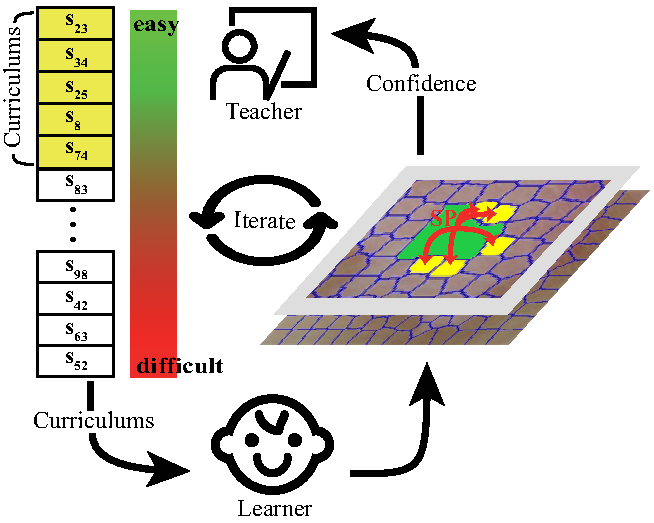
\includegraphics[width=0.7\linewidth]{TLLTillustrator.pdf}
\end{center}
\caption{显着性传播过程。在左侧,教师选择几个最简单的节点(黄色)作为学习者的课程。然后,学习者通过显着性传播“学习”这些节点。在右侧,学习者向教师提供反馈(即信心),以帮助教师确定下一个课程的数量。}
\label{fig:TLLTillustrator}
\end{figure}

显著性传播方法在我们的算法中非常重要. 假设我们在图$\mathcal{G}$中有$l$个种子节点$\mathbf{s}_1,\cdots , \mathbf{s}_l$, 其值为$f_1=\cdots = f_l =1$, 显著性传播的任务是将显著性值准确可靠从这些已经标记的$l$个节点传播到剩余的$u=N-l$个未被标记的超像素。
然而现有方法的传播顺序可能在处理较复杂的超像素时产生瑕疵,所以本文基于自动控制原理中的反馈思想,在原先框架上优化学习顺序(见图\ref{fig:TLLTillustrator})。

具体来说,这个框架由学习者和教师组成。 给定在时间$t$标记的集合$\mathcal{L}^{(t)}$和未标记的集合$\mathcal{U}^{(t)}$,老师从中$\mathcal{U}^{(t)}$选择一组简单的超像素作为为课程$\mathcal{T}^{(t)}$。 然后,学习者将学习$\mathcal{T}^{(t)}$,并将反馈返回给老师以帮助老师更新$(t + 1)$次学习的课程。 这个过程迭代直到$\mathcal{U}^{(t)}$中的所有超像素都被传播到。

\subsection{``教学''过程}
``教学''过程的核心在于设计一个老师,这个老师可以决定哪些未被标记的超像素在接下来的过程中被学生学习。对于第$t$次传播过程,首先建立一个候选集$\mathcal{C}^{(t)}$,其中元素是在图$\mathcal{G}$中直接与$\mathcal{L}^{(t)}$相邻的超像素。然后教师从$\mathcal{C}^{(t)}$中选择最简单的几个元素作为第$t$次的课程。为了衡量超像素$\mathbf{s}_i \in \mathcal{C}^{(t)}$ 的传播难度,我们定义难度系数$DS_i$
\begin{equation}
DS_i=INF_i+IND_i+IHM_i+CON_i
\end{equation}
其中$INF_i$度量信息性,$IND_i$度量个体性,$IHM_i$度量不同质性,$CON_i$度量连通性。接下来本文详细的介绍每一种度量的定义。

\textbf{信息性:}在给定集合$\mathcal{L}$之后,简单的超像素不应该再引入过多的信息,于是一个超像素$\mathbf{s}_i \in \mathcal{C}$的信息性度量可以直接使用条件熵$H(\mathbf{s}_i \mid \mathcal{L})$进行建模,表示为:
\begin{equation}
INF_i=H(\mathbf{s}_i \mid \mathcal{L})
\end{equation}
这个传播过程遵循多元高斯过程,在随机向量$\mathbf{f}=(f_1 \cdots f_N)^ \mathrm{T}$中的元素$f_i(i=1, \cdots ,N)$代表超像素$\mathbf{s}_i$的显著值。相关协方差矩阵$\mathbf{K}$相当于将邻接矩阵$\mathbf{W}$的对角线元素全部置为$1$.
对于多元高斯,$H(\mathbf{s}_i \mid \mathcal{L})$闭式表达为:
\begin{equation}
INF_i=H(\mathbf{s}_i \mid \mathcal{L})=\frac{1}{2}\ln{(2 \pi e \sigma_{i \mid \mathcal{L}}^2)}
\end{equation}
其中$\sigma_{i \mid \mathcal{L}}^2$是给定$\mathcal{L}$后$f_i$的条件协方差,考虑到条件分布是一个多元高斯,$\sigma_{i \mid \mathcal{L}}^2$可以表达成
\begin{equation}
\label{eq:7}
\sigma_{i \mid \mathcal{L}}^2=\mathbf{K}_{ii}^2-\mathbf{K}_{i,\mathcal{L}} \mathbf{K}_{\mathcal{L},\mathcal{L}}^{-1} \mathbf{K}_{\mathcal{L},i},
\end{equation}
其中$\mathbf{K}_{i,\mathcal{L}} $和$\mathbf{K}_{\mathcal{L},\mathcal{L}} $表示$\mathbf{K}$的子矩阵。通过带入消元,我们得到$\mathbf{s}_i$
在\eqref{eq:7}中对$\mathbf{K}_{\mathcal{L},\mathcal{L}}$求逆的步骤在每一次迭代过程都需要进行计算,随着集合$\mathcal{L}$越来越大,直接求逆非常的耗费时间,因此一种高效的基于块的更新方法在补充材料中进行了推导。

\textbf{个体性:} 个体性衡量一个超像素与其周围邻居超像素有多么不同.我们认为一个简单的超像素与周围的超像素具有相似的LAB 颜色空间。一个超像素个体性度量越小,则说明与其周边超像素越相近。
\begin{equation}
\label{eq:8}
IND_i=IND(\mathbf{s}_i,{\mathcal{N}(\mathbf{s}_i)})=\frac{1}{|\mathcal{N}(\mathbf{s}_i)|}\sum_{j\in \mathcal{N}(\mathbf{s}_i)}\| \mathbf{s}_i^{\mathrm color}-\mathbf{s}_j^{\mathrm color}\|,
\end{equation}
其中$\mathcal{N}(\mathbf{s}_i)$表示$\mathbf{s}_i$邻居的数目

\textbf{同质性:}显然,对于一个不同质的超像素来说,其中包含的像素是多样的、不统一的。假设在超像素$\mathbf{s}_i$中有$b$个像素$\{\mathbf{p}_j^{\mathrm color}\}^b_{j=1}$,向量的维度代表LAB颜色特征。然后将他们的相关性记录在一个$b \times b$的对称矩阵$\pmb{\Theta}=\mathbf{P}\mathbf{P^{\mathrm T}}$,其中矩阵$\mathbf{P}$的每一行代表了一个像素的特征向量$\mathbf{p}_j^{\mathrm color}$的转置,因此超像素$\mathbf{s}_i$的$IHM_i$定义为:
\begin{equation}
\label{eq:9}
IHM_i=\Big (\frac{2}{b^2-b}\sum_{i=1}^b \sum_{j=i+1}^b\pmb{\Theta}_{ij}\Big )^{-1}
\end{equation}
其中$\pmb{\Theta}_{ij}$是矩阵$\pmb{\Theta}$的第$(i,j)$个元素,一个较小的$IHM_i$意味着超像素$\mathbf{s}_i$中的所有像素都很相似,并且可以很容易被学习者学习。

\textbf{连通性:}对于已经建立的图$\mathcal{G}$来说,一个直觉是与集合$\mathcal{L}$连接性强的超像素并不难进行传播。于是超像素$\mathbf{s}_i \in \mathcal{C}$与集合$\mathcal{L}$中的所有元素的测地距离与其连通性度量成反比例关系。
\begin{equation}
\label{eq:10}
CON_i=\frac{1}{l}\sum_{j\in \mathcal{L}}\mathrm{geo}({\mathbf{s}_i,\mathbf{s}_j})
\end{equation}
在\eqref{eq:10}中,$\mathrm{geo}({\mathbf{s}_i,\mathbf{s}_j})$表示$\mathbf{s}_i$与$\mathbf{s}_j$之间的测地距离,可以使用最短路径进行近似:
\begin{IEEEeqnarray}{rCl}
\label{eq:11}
\mathrm{geo}({\mathbf{s}_i,\mathbf{s}_j})&=\min_{R_1=i,R_2,\cdots,R_n=j}\sum_{k=1}^{n-1}\max{({E_{R_k,R_{k+1}}-c_0},0)}  \\
\mathrm{s.t.} & R_k,R_{k+1} \in \mathcal{V}, R_k\mbox{和}R_{k+1}\mbox{相邻} \nonumber
\end{IEEEeqnarray}
此处$\mathcal{V}$代表$\mathcal{G}$的顶点集,$E_{R_k,R_{k+1}}$计算了$R_k$和$R_{k+1}$的欧式距离,其中$c_0$是一个自适应阈值,用来防止``小权重积累问题''.

最终,通过公式代换,我们得到了所有$\mathbf{s}_i \in \mathcal{C}$的难度系数,在老师的帮助下,未被标记的超像素逐渐从简单到复杂的学习。

\subsection{反馈过程}
在计算了所有候选超像素的难度系数之后,下一步便是选取特定数量的超像素作为课程。一个直接的想法是,将元素从小到大排序后选择前$q \,(q\leq |\mathcal{C}|)$个用来建立课程集合$\mathcal{T}=\{\mathbf{s}_1,\mathbf{s}_2,\cdots,\mathbf{s}_q\}$但我们认为在第$t$次所学的数目应该由第$t-1$次所学效果决定:如果第$t-1$次学习过程比较自信,那么教师会分派更多的学习任务给学习者。也就是说,教师应该考虑学习者的反馈来调节课程量。于是我们使用自适应的$q^{(t)}$作为第$t$次所学的课程量。

正如上面所讲,$q^{(t)}$应该被前一次的学习过程所决定。但是因为第$t-1$次学习的正确性无从得知,于是本文定义了置信值来估计此前的学习效果。直观上讲,如果显著值$f_1^{t-1},\cdots, f_{q^{(t-1)}}^{(t-1)}$在归一化之后接近$0$\,(与种子点非常不相似)\,或者$1$\,(与种子点极为相似),则认为第$t-1$次学习的置信度高,相反如果$f_1^{t-1},\cdots, f_{q^{(t-1)}}^{(t-1)}$接近$0.5$,这意味着此学习的置信度低,于是第$t$次应该使用一个更小的$q^{(t)}$。于是置信度(属于$[0,1]$之间)定义为:
\begin{equation}
\label{eq:12}
\mathrm{ConfidenceScore}=1-\frac{2}{q^{(t-1)}}\sum_{i=1}^{q^{(t-1)}}\min{(f_i^{(t-1)},1-f_i^{(t-1)})}, 
\end{equation}
最终可以计算出来$q^{(t)}$:
\begin{equation}
\label{eq:13}
q^{(t)}={|\mathcal{C}^{(t)}|\times \mathrm{ConfidenceScore}}.
\end{equation}

\subsection{显著性传播过程}
当课程$\mathcal{T}=\{\mathbf{s}_1,\mathbf{s}_2,\cdots,\mathbf{s}_{q^{(t)}}\}$确定了之后,学习者通过传播过程将显著值从$\mathcal{T}^{(t)}$传播到$\mathcal{L}^{(t)}$,可表达为:
\begin{equation}
\label{eq:14}
\mathbf{f}^{(t+1)}=\mathbf{M}^{(t)}\mathbf{D}^{-1}\mathbf{W}\mathbf{f}^{(t)}
\end{equation}

其中$\mathbf{M}$是一个对角线矩阵,如果$\mathbf{s}_i\in \mathcal{T}^{(t)}\cup \mathcal{L}^{(t)}$,
那么令$\mathbf{M}_{ii}^{(t)}=1$,否则$\mathbf{M}_{ii}^{(t)}=0$,当第$t$步迭代完成了之后,被标记和未被标记的集合更新为$\mathcal{L}^{(t+1)}=\mathcal{L}^{(t)} \cup \mathcal{T}^{(t)}$,$\mathcal{U}^{(t+1)}=\mathcal{U}^{(t)} \setminus \mathcal{T}^{(t)}$.

以$\mathbf{f}^{(0)}=\Big (f_1^{(0)},\cdots,f_N^{(0)}\Big)$初始化公式\ref{eq:14}, 如果第$i$个超像素对应于种子点,则令$f_i^{(0)}=1$,否则令$f_i^{(0)}=0$。当集合$\mathcal{U}$为空时终止,得到显著值向量$\mathbf{f}$。

\section{实验结果与分析}
在本节中,首先在定性上将本文的方法与TLLT \cite {gong2015saliency}进行比较,并说明本文的优势。然后,定性和定量地比较本文的方法与现有技术,并讨论失败的案例。然后进行简化模型研究,即通过化简模型来讨论模型中每一个步骤的必要性,并进行参数灵敏度分析。本文在整个实验中使用以下参数:$ {N_\mathrm {max}} = 400, T_\mathrm {f} = 30, {T_ \mathrm {b}} = 60, \theta = 0.25, \eta = 0.4 $ 。


\subsection{注意力机制验证}
在\cite{gong2015saliency}中,凸包提取与检测用于粗略定位特征对象。然而,它总是具有误导性(见图 \ref {fig:TLLT}),因为与面部的其他部位(例如,鼻子,嘴唇,眉毛,眼睛)相比,白癜风不是一个显着的对象。相比之下,本文从类感知激活图中引入了先验,这可以帮助我们正确地关注于我们关心的对象。

\begin{figure}[htbp]
\begin{center}
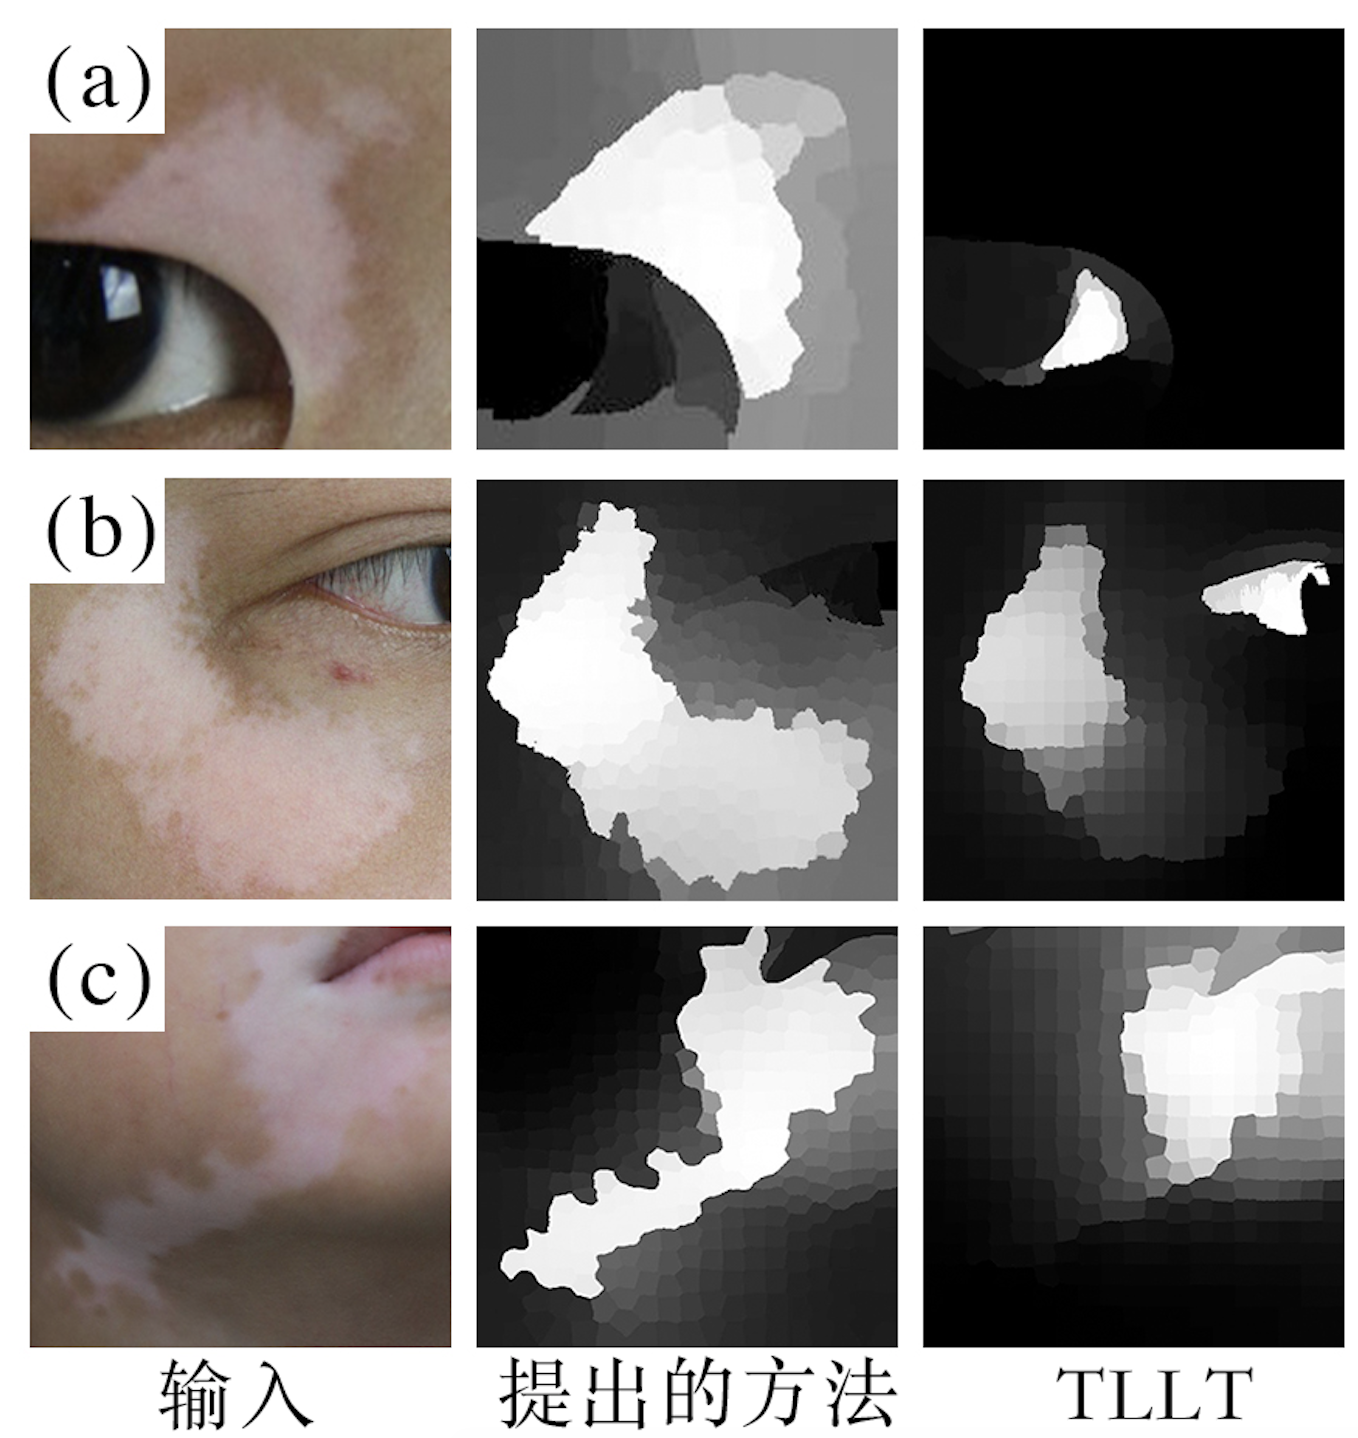
\includegraphics[width=0.6\linewidth]{TLLT.png}
\end{center}
\caption{与TLLT的效果对比。在每行中,从左到右的图像分别代表原始图像、本文的方法的结果和TLLT的结果。 (a)和(b)显示TLLT专注于错误的地方,而本文的方法可以正确地专注于白癜风区域。(c)显示本文的方法可以很好地抑制背景并使前景脱颖而出。}
\label{fig:TLLT}
\end{figure}

为了逐渐将注意力集中在我们感兴趣的物体上,本文通过引入几个先验来抑制背景,从而使前景突出。为了量化这个过程,本文借用了信噪比的概念。也就是说,根据真值图像,显着性值位于白癜风区域被认为是一个有用的信号,而显着性值在非白癜风区域则被视为无用的噪音信号。我们将其表述为:
\begin{equation}
\label{eq:16}
\mathrm{SNR_{dB}}=10\mathrm{log_{10}}(\frac{E_{\mathrm{signal}}}{E_{\mathrm{noise}}}),
\end{equation}

其中 $E_\mathrm{signal}$ 和 $E_\mathrm{noise}$ 分别是信号和噪声的能量项, 由显著性值的均方差所度量。 统计结果参见图\ref{fig:SaliencySNR}. 如果将 $\mathrm{SNR_{dB}}=0$ 作为基准线,可以发现在引入先验之后,显著性图的信噪比$S_\mathrm{Bg}$ 和 $S_\mathrm{Bnd}$均有所增加。然后通过结合细化显著性图的步骤,我们最终得到的显著性图$S_\mathrm{Final}$的信噪比有了非常大的提升($2.08$ dB)。
 
\begin{figure}[htbp]
\begin{center}
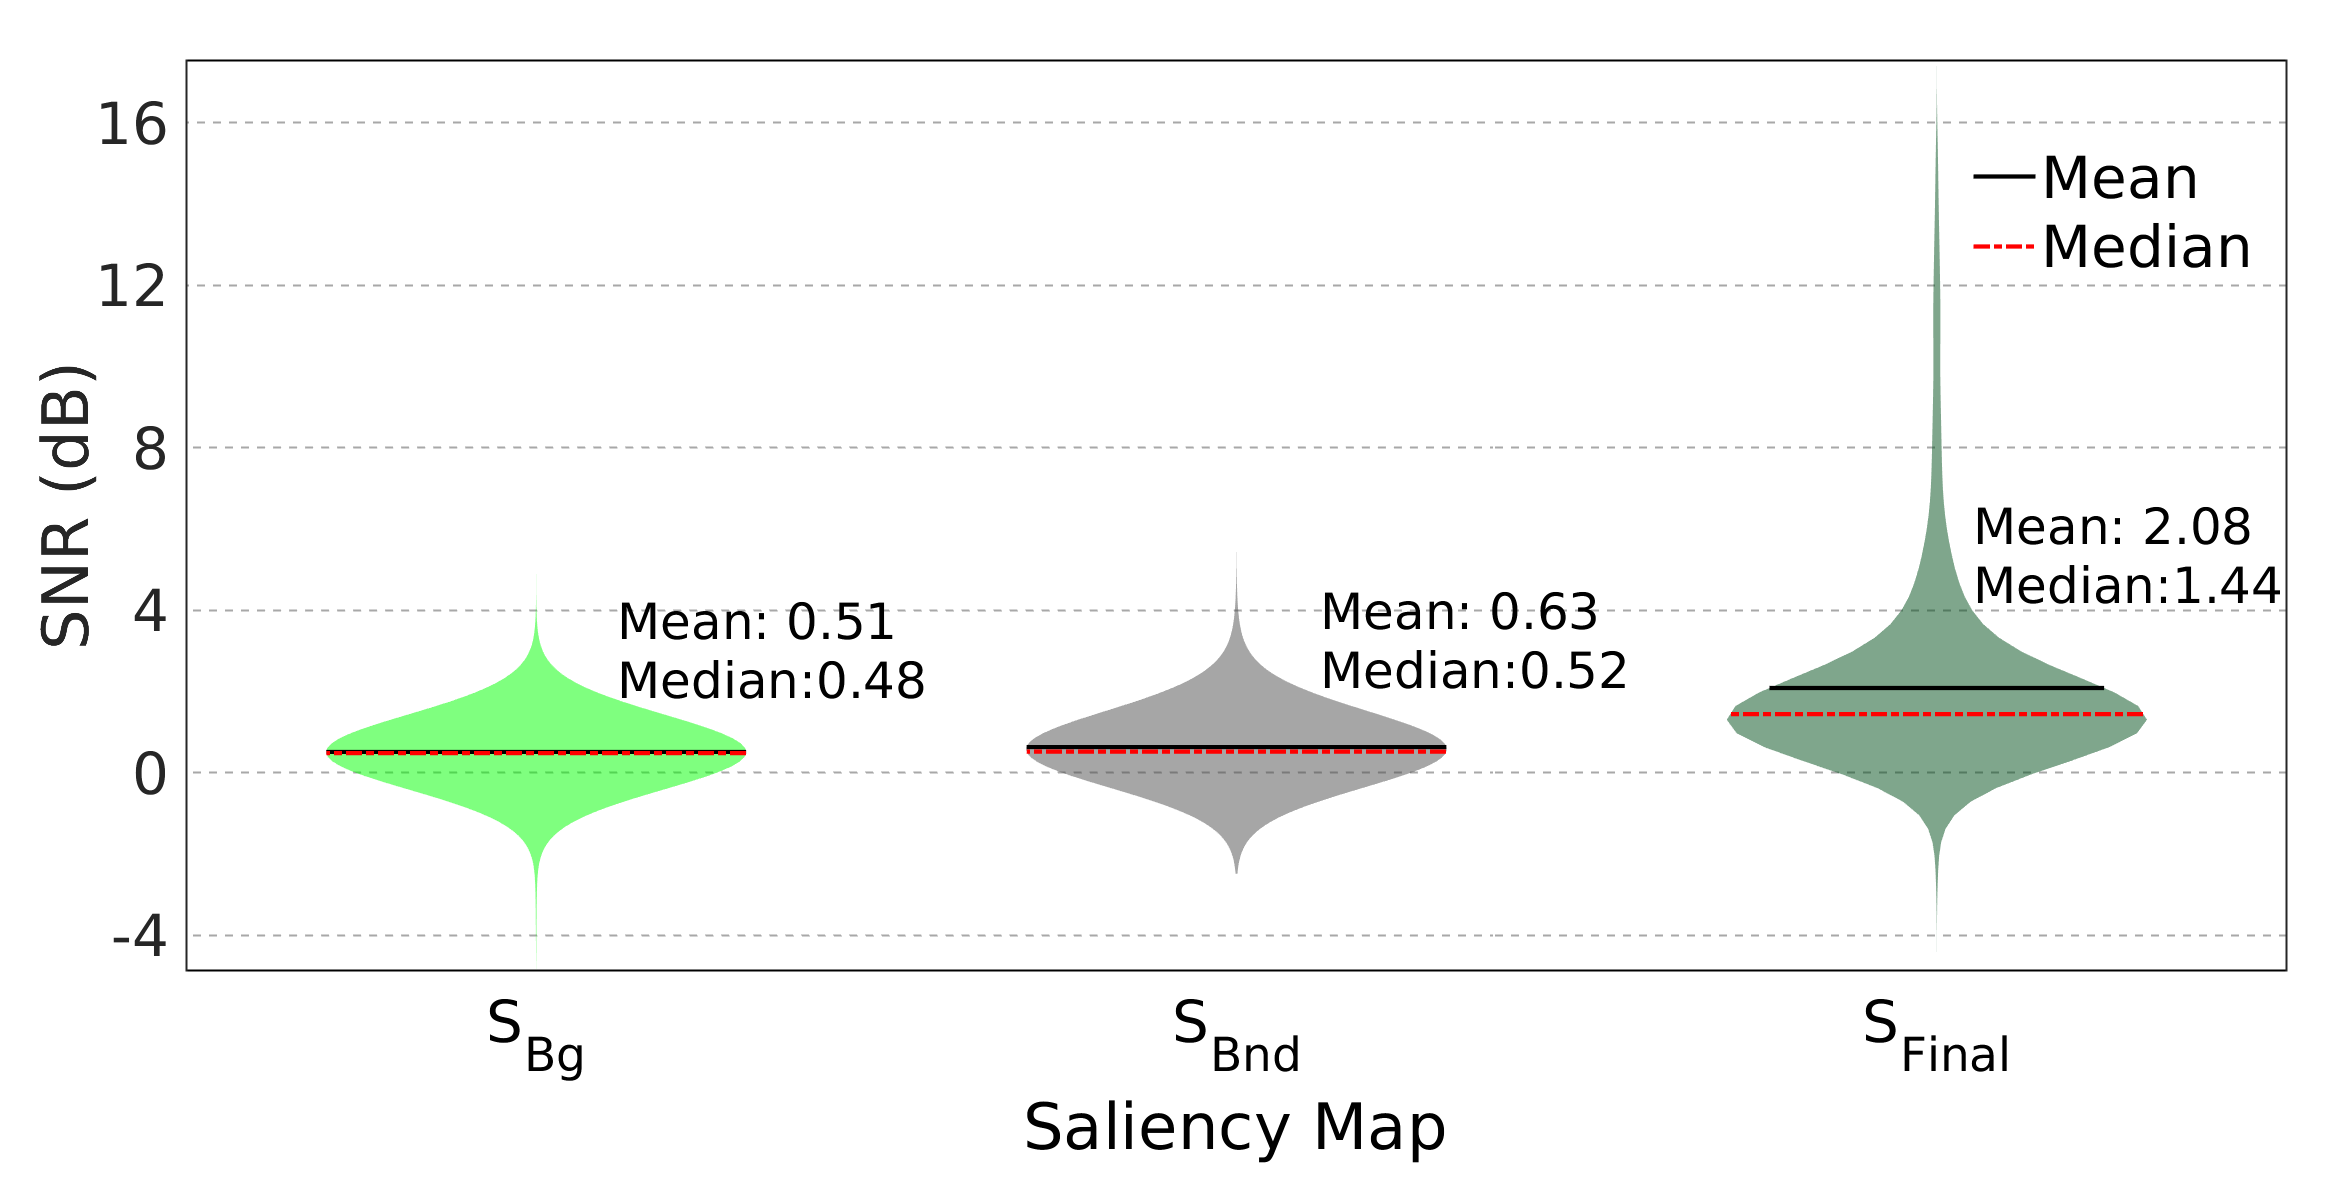
\includegraphics[width=0.8\linewidth]{VitViolin.eps}
\end{center}
\caption{三个显著性图的信噪比,即 $S_\mathrm{Bg}$, $S_\mathrm{Bnd}$ 和 $S_\mathrm{Final}$.}
\label{fig:SaliencySNR}
\end{figure}

\subsection{分割效果的定量与定性分析}
\textbf{定量分析}

给定输入图像,本文的算法产生具有若干灰度级的显著图。为了与不同的分割方法进行比较,设置阈值($ {T_ \mathrm {bin}} = 0.5 $)最终获得二元掩模。本文采用IoU来评估算法的性能。

\begin{table}[tbp]
  \begin{center}
  \caption{全监督学习与弱监督学习在Vit2019数据集上的表现,以IoU (\%)为衡量标准}
    \begin{tabular}{c|c|c}
    \toprule
   方法 & 监督形式 & mIoU \\
    \hline
    \hline
    FCN-VGG16\cite{long2015fully}  & \multirow{2}[2]{*}{Fully} & 72.4 \\
    U-net\cite{ronneberger2015u} &       & 78.6 \\
    \hline
    PRM\cite{Zhou:2018ul}   & \multirow{3}[2]{*}{Weakly} & 67.2 \\
    SEC\cite{Kolesnikov:2016tf}   &       & 64.7 \\
    Our Method &       &\textbf{71.4}\\
    \bottomrule
    \end{tabular}%
\end{center}
  \label{tbl:CompareResult}%
\end{table}%

在表4.1中,本文首先将两种典型的完全监督方法U-net和FCN在Vit2019上进行测试,然后与最先进的弱监督方法进行比较,即 \cite{Zhou:2018ul, Kolesnikov:2016tf}。本文的方法使用图像级标签和标准设置来训练分类模型,而没有使用CRF后处理\cite{Kolesnikov:2016tf}或生成可能的切割面片的方法\cite{Zhou:2018ul},并通过阈值操作直接生成二进制掩码并显现了有竞争力的结果。可以看出,本文的方法在一定程度上优于其他弱监督方法,并减小了弱监督和全监督方法效果之间的差距。

\textbf{定性分析}

首先,与表4.1中的完全监督方法相比,虽然本文的表现一般较差,但在一些具有挑战性的图片中,本文的方法优于U-net,如图~\ref {fig:unetResult}。在低对比度条件下,本文的方法可以更好地定位皮肤病变区域,显著图本身可以更好地反映健康皮肤和白癜风皮肤之间的过渡区域。对于包含毛发脱色的部分,也可以在得到的二元掩模图像中得到反映。对于某些高光区域,例如嘴唇上的反射,我们的方法也可以降低误报率。而且,我们的方法可以更好地保留边缘的细节。

\begin{figure}[htbp]
\begin{center}
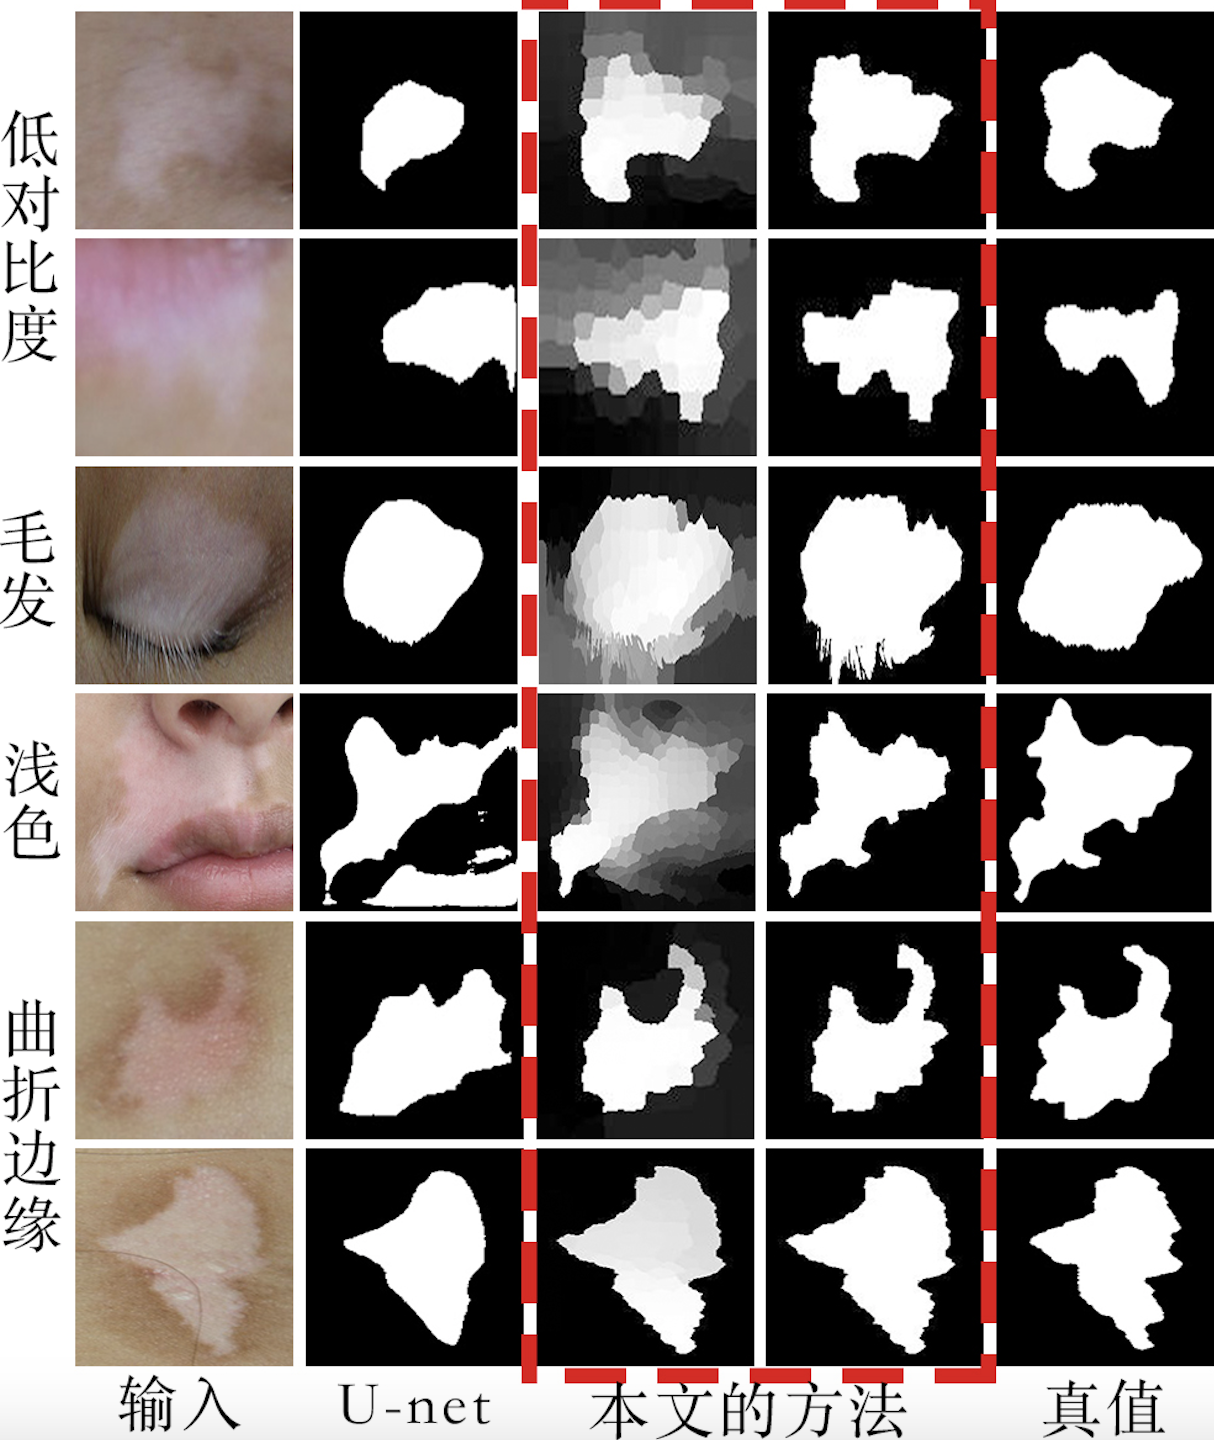
\includegraphics[width=0.7\linewidth]{unetcompareSmaller.png}
\end{center}
   \caption{U-net和我们的方法生成的掩码的可视化比较。在使用$ {T_ \mathrm {bin}} $对本文方法所获得的显着性图(红色虚线框中的第一列)进行阈值处理后,我们可以获得二元掩模(框中的第二列)。真值(GT)在最后一栏中给出。}
\label{fig:unetResult}
\end{figure}

其次,与最先进的弱监督方法相比,如图\ref {fig:weaklySupervisedCompare}所示,我们的方法可以保持较好的边界,并在恶劣条件下保持鲁棒性。

\begin{figure}[h]
\begin{center}
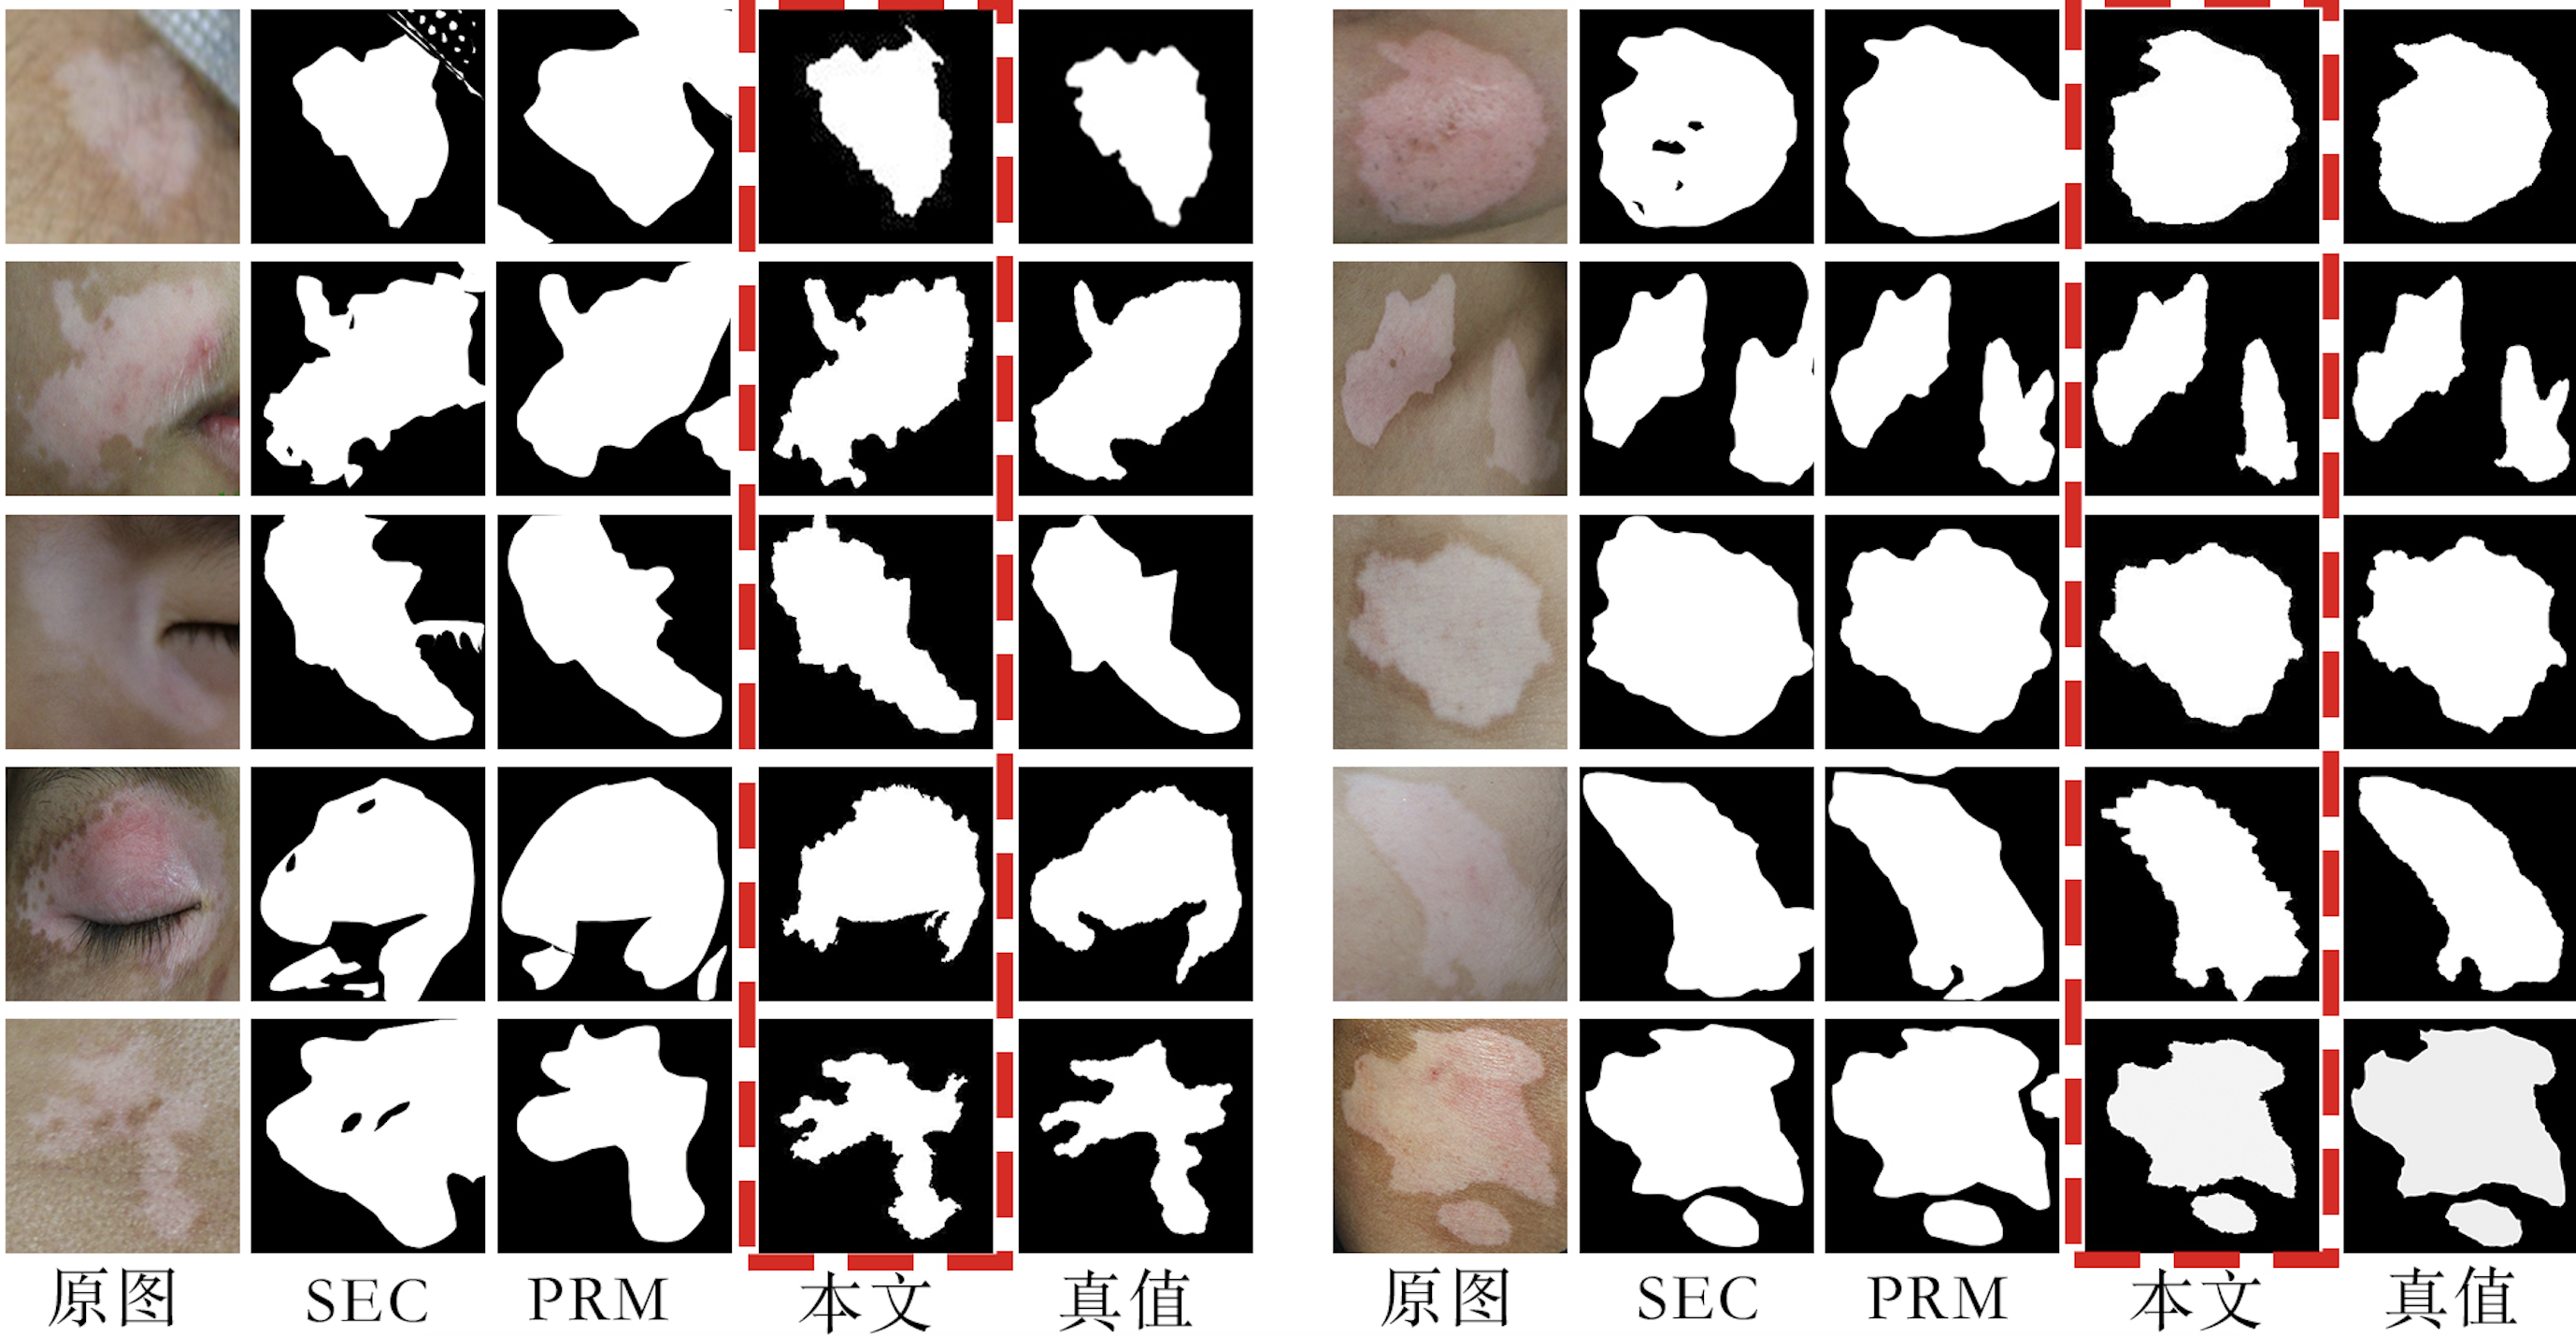
\includegraphics[width=\linewidth]{weaklySupervisedCompare.png}
\end{center}
   \caption{本文的方法与最先进的弱监督方法之间的视觉比较,即 SEC~\cite{Kolesnikov:2016tf} 和 PRM~\cite{Zhou:2018ul}. }\vspace{-3mm}
\label{fig:weaklySupervisedCompare}
\end{figure}

我们的失败的情况主要是由于在低对比度的情况下下,全局阈值$ {T_ \mathrm {bin}} $不恰当的设置(参见图\ref {fig:FailureCases})。然而,在真实的临床场景中,由于白癜风的性质,我们的显着图中的灰度级可以更好地代表皮损与健康皮肤之间的过渡区,并有助于评估不同程度的脱色素。此外,本文的方法有时会在强烈的光照条件下将正常皮肤误判为白癜风区域。

\begin{figure}[h]
\begin{center}
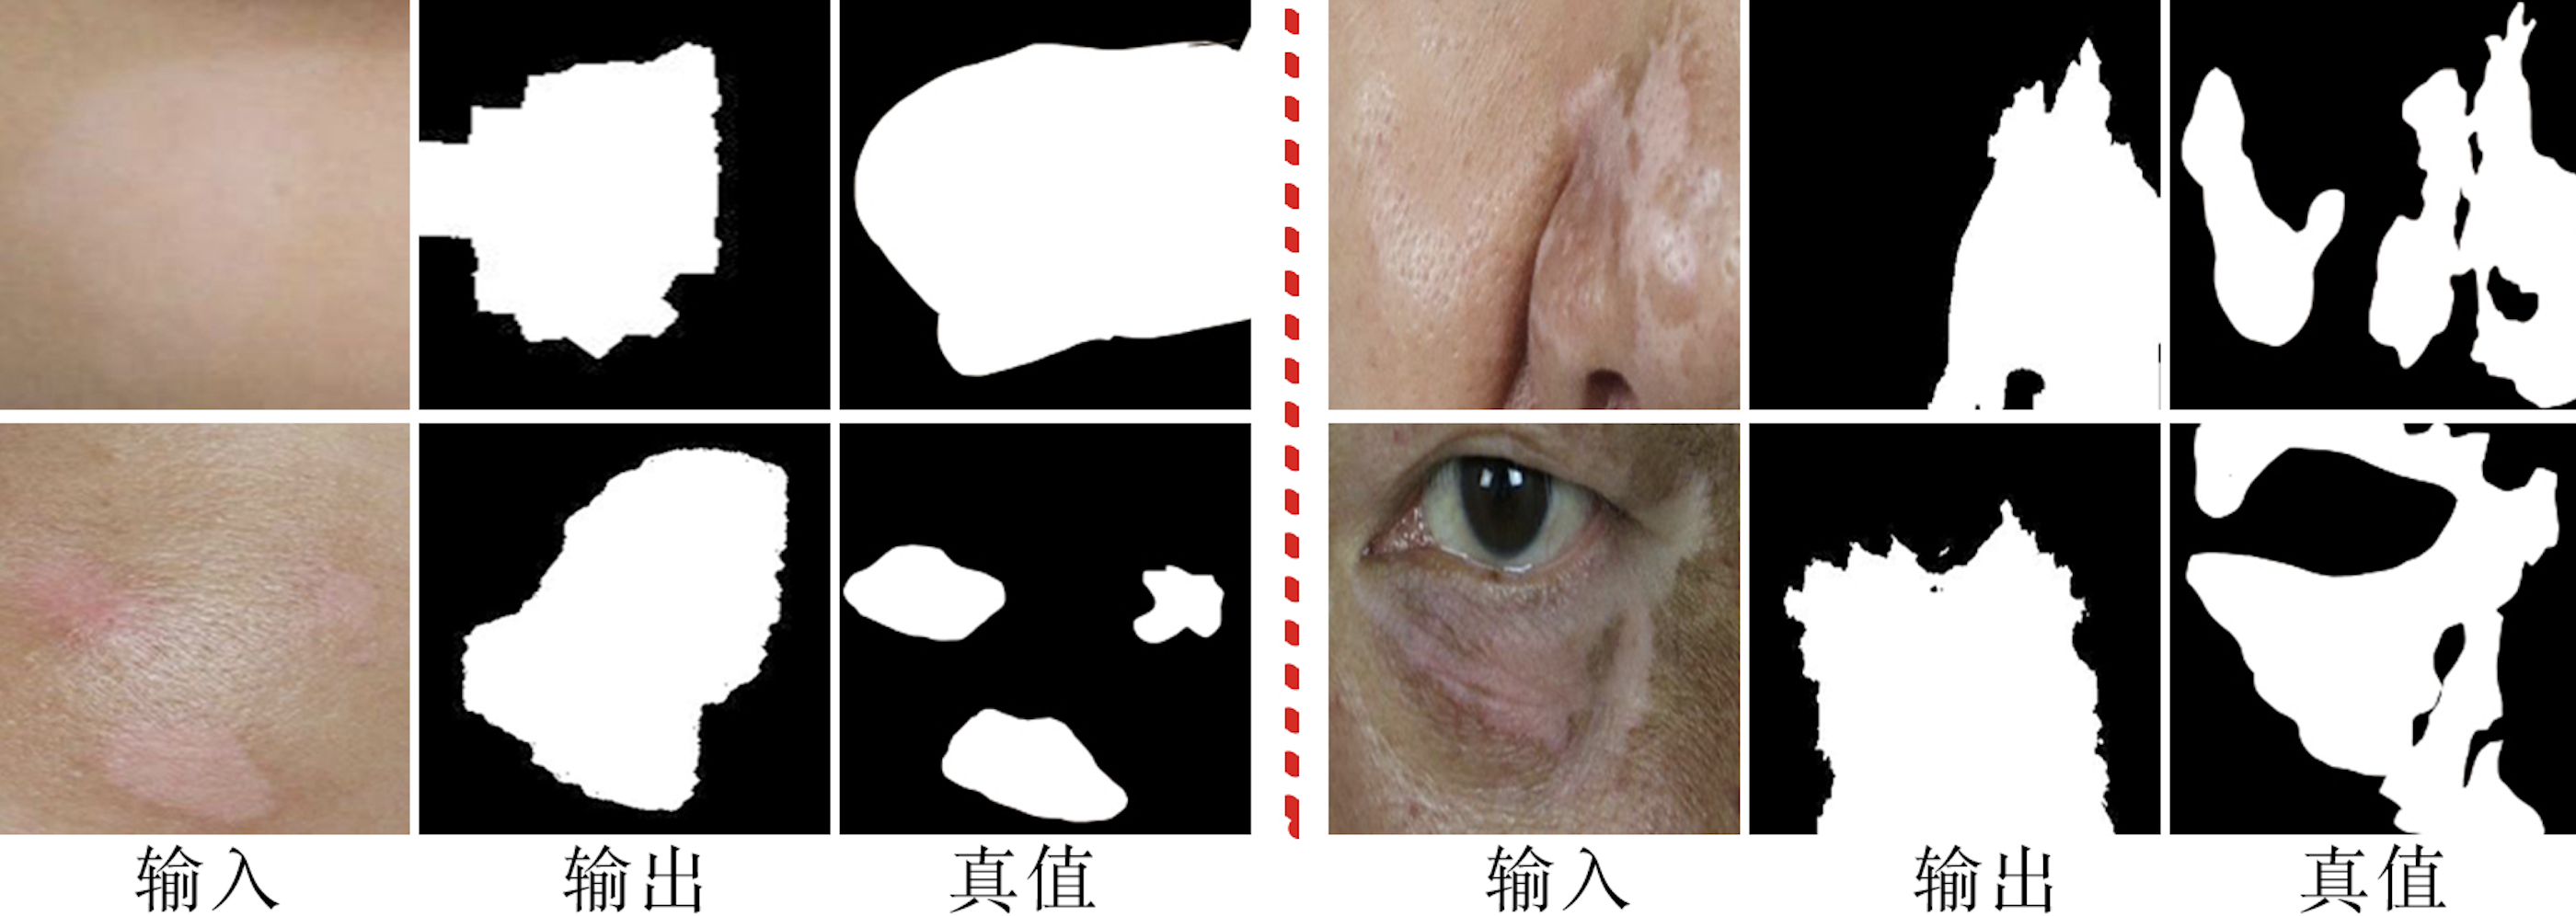
\includegraphics[width=\linewidth]{FailureCases.png}
\end{center}
   \caption{失败的案例}
\label{fig:FailureCases}
\end{figure}

\subsection{模型简化研究与敏感性测试}
\textbf{模型简化研究}


基于之前的介绍,本文总共引入了三个先验知识来帮助我们获得最终的显着性图,即前景蒙版,背景种子和边界种子。为了研究每个先验知识的贡献,我们在表4.2中探索了不同的组合所产生的结果。可以得出以下结论:

\begin{enumerate}
\item 当省略前景掩模和背景种子时,mIoU分别从71.4\%下降到62.5%和66.7\%,这表明激活图产生的先验的有效性。
\item 引入边界种子使性能提高了8.3\% 表明假设边界像素主要来自背景区域是有帮助的。
\item 当去掉三个先验中的两个时,mIoU从71.4\%急剧下降到59.5\%,43.5%和53.0\%,这表明三个先验是不可或缺的。
\item 当我们不使用最后一个显着性传播过程(同时丢弃前景掩码)并直接使用$ {T_ \mathrm {bin}} $来阈值分割$ S_\mathrm {Bnd} $和$ S_ \mathrm {Bg} $的乘法结果时,最终产生的二进制掩码与仅丢弃前景掩码相比IoU下降了4.8\%,这表明最后的显着性传播过程可以进一步提高显著图的质量。
\end{enumerate}

\begin{table}[htbp]
\label{tab:ablation}
\begin{center}
\caption{简化模型分析:针对不同的先验知识与显著性传播过程}
\setlength{\tabcolsep}{1 mm}{
    \begin{tabular}{c|cccccccc}
    \toprule
    Fg Mask & \xmark &   \cmark    &    \cmark   &   \cmark    & \xmark & \xmark & \xmark & \cmark \\
    Bg Seeds &  \cmark     & \xmark &   \cmark    & \xmark &  \cmark     & \xmark &  \cmark     & \cmark \\
    Bnd Seeds &  \cmark     &   \cmark    & \xmark & \xmark & \xmark &   \cmark    &   \cmark    & \cmark \\
    Last SP &   \cmark    &   \cmark    & \cmark      &   \cmark    &  \cmark     &    \cmark   &\xmark & \cmark \\
    \midrule
    mIoU  & 62.5  & 66.7  & 63.1  & 59.5  & 43.5  & 53.0  & 57.7  & \textbf{71.4}  \\
    \bottomrule
    \end{tabular}}%
\end{center}

  \label{tab:ablation}%
\end{table}%

\textbf{敏感性测试}

本文的算法中一共有五个参数需要手动调节,高斯核宽度$\theta$, 最大的超像素数量 ${N_\mathrm{max}}$, 二值化阈值 ${T_\mathrm{bin}}$,用于细化显著图的选择率 $\eta$ 以及用于获得前景与背景掩模的阈值对 $(T_\mathrm{f}$-$T_\mathrm{b})$ 。我们在此过程中使用控制变量法,在 $\mathrm{IoU}$意义下评估了每一个参数对模型的影响。图~\ref{fig:Sensitivity} 显示了本文的方法对于$\eta$ 和 ${N_\mathrm{max}}$的改变并不敏感,但是性能却非常依赖于 $\theta$的选择。 ${T_\mathrm{bin}}$ 的变化在以 $0.5$为中心的一个较大区间内变化均可以被接受。经过大量的实验,发现本文的方法具有很强的鲁棒性, 并且对于阈值对$(T_\mathrm{f}$-$T_\mathrm{b})$的选择在很大一个自由区间内仍然可以维持算法的有效性。经过测试,本文算法的最佳性能在取${T_\mathrm{b}}=30,{T_\mathrm{f}}=60$时达到。

\begin{figure}[htbp]
\begin{center}
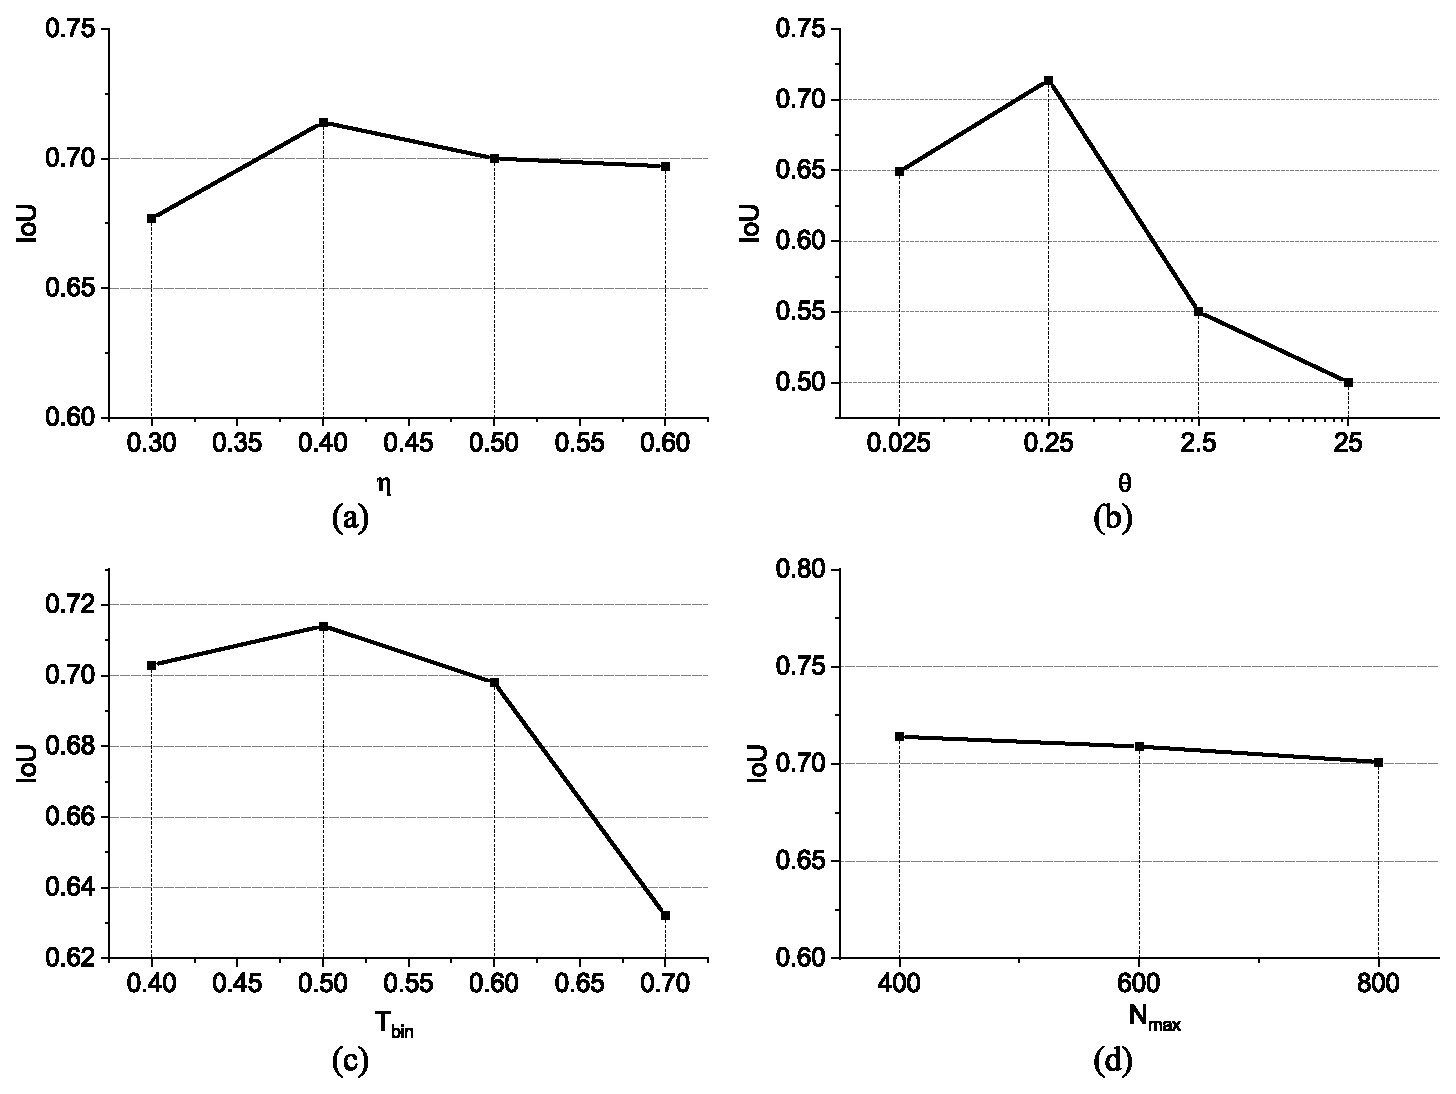
\includegraphics[width=0.7\linewidth]{composit1.eps}
\end{center}
   \caption{敏感性测试}
\label{fig:Sensitivity}
\end{figure}


\section{本章小结}
本章首先分析了在医疗图像处理领域对图像真值标注的困难性,然后引出了弱监督学习、弱监督分割的概念。然后提出了本文的核心方法并分别详细介绍了每一步骤中的原理以及意义,解释了如何做到“既见森林,又见树木”,解释了如何将反馈的思想应用到显著性传播的过程中,并说明了这种策略应用在白癜风分割领域所带来的好处。最后通过多个实验验证了该方法的有效性,并与强监督学习进行对比,发现在一些拍照环境恶劣,对比度很低的情况下,本文提出的方法可以更好的保持白癜风的边缘。



















